\documentclass[main.tex]{subfiles}
\begin{document}

\chapter{Implementation}
In order to support the proof of concept for the model as proposed in chapter \ref{chapter:model}, a number of the model's parts have been implemented:
\begin{itemize}
    \item Experiment setup package specification
    \item Experiment setup wrapper
    \item Digilent Nexys 4 controller
    \item Experimentation package specification
    \item Digilent Nexys 4 composer
\end{itemize}

As discussed while establishing the thesis' scope in section \ref{section:scope}, this thesis goal is not to achieve platform independence. As such, the implementation is specifically targeted at the Digilent Nexys 4 development board and the toolchain offered by the Xilinx Vivado HL WebPack edition, version 2016.1. The possibilities of achieving platform indepence are discussed in section \ref{section:futurework}.

\section{Experiment Setup Package Specification}
\label{section:experiment-setup-package-specification}
A format for the model's experiment setup package has been defined. For the purposes of portability, a \texttt{.zip} archive is used as a means for containment of all associated files. A manifest file describes the contents of the package. This approach to packaging was derived from other packaging methods, such as java \texttt{.jar} packages. Figure \ref{fig:experiment-setup-package-filesystem} displays an overview of the experiment setup package file structure. The name and location of the manifest file is constrained by the specification, but the names and structure of other files contained in the package are not limited by any constraints.

\begin{figure}[h]
\centering
\caption{An overview of the experiment setup package file structure}
\label{fig:experiment-setup-package-filesystem}
\begin{subfigure}[b]{0.4\textwidth}
\dirtree{%
.1 package.zip.
.2 directory/.
.3 directory/.
.4 \dots.
.3 source file. 
.3 \dots.
.2 source file. 
.2 \dots.
.2 mainfest.yaml. 
}
\end{subfigure}
\end{figure}

The manifest file describes the contents of the experiment setup package and its information is encoded in \texttt{YAML}\footnote{http://yaml.org/} syntax, a widespread format for capturing configuration information. Besides package metadata, such as title and author information, the manifest also contains file pointers and a description of the experiment setup's address space. Furthermore, the manifest defines the widths for the address and data buses. The contents of an example experiment setup package manifest file are displayed in listing \ref{lst:experiment-setup-package-manifest}. In automated processes, this manifest file is generated by the experiment setup wrapper, as described in section \ref{section:experiment_setup_wrapper}.

\begin{lstlisting}[caption={Example experiment setup package \texttt{manifest.yaml}}, label={lst:experiment-setup-package-manifest}]
title: Full Adder using Half
description: >
    An implementation of a full adder using two half adders.
author: Matthijs Bos
date: (*@ \today @*)
url: https://github.com/matthijsbos/fulladderhalf/
vhdlFfiles: 
    - wrapper.vhd
    - fulladder.vhd
    - halfadder.vhd
topLevelFile: ./wrapper.vhd
addressWidth: 3
dataWidth: 1
addressSpacePartitioning:
    - { name: a,    direction: in,  address: 0x0, width: 1 }
    - { name: b,    direction: in,  address: 0x1, width: 1 }
    - { name: cin,  direction: in,  address: 0x2, width: 1 }
    - { name: s,    direction: out, address: 0x3, width: 1 }
    - { name: cout, direction: out, address: 0x4, width: 1 }
\end{lstlisting}






\section{Experiment Setup Wrapper}
\label{section:experiment_setup_wrapper}
A tool has been developed to automate the model's experiment setup wrapping process, as described in section \ref{sectionexperimentsetupwrapping}. The tool has been implemented using the Java 8 programming language and its source code is made available through a git repository\footnote{\url{https://github.com/matthijsbos/fpgaedu-java}}. This tool takes an existing VHDL implementation and a configuration file to automatically generate an experiment setup package. The tool is activated through the command line by the command \texttt{fpgaedu wrap}.
% , as shown in figure \ref{fig:wrapper-overview}. 

% \begin{figure}[h]
%     \centering
%     \caption{An overview of the experiment setup wrapper operation}
%     \label{fig:wrapper-overview}
%     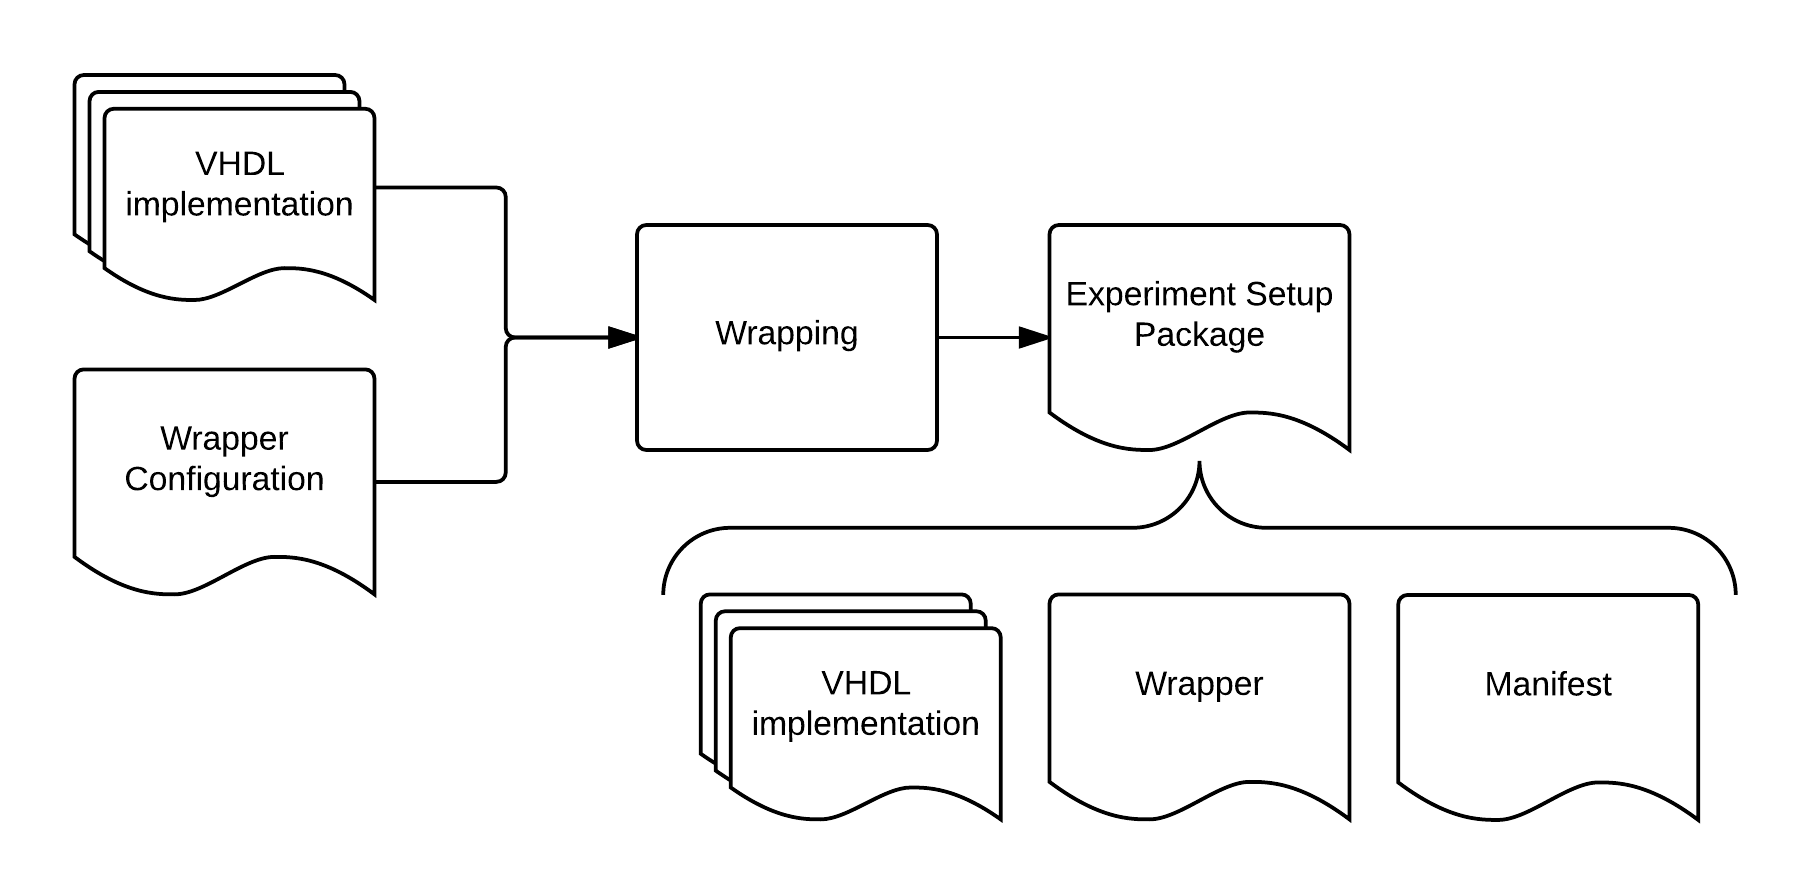
\includegraphics[width=0.7\textwidth]{img/wrapper}
% \end{figure}

Listing \ref{lst:wrapper-configuration} displays an example configuration file for the wrapper tool. This file contains contains pointers to the VHDL files that define the experiment setup's implementation as well as a pointer to the file that contains the implementation's top-level module. Additionally, the configuration file is also used to specify experiment setup metadata entries which are copied into the experiment setup package's manifest file. 

\begin{lstlisting}[caption={Example \texttt{fpgaedu.yaml} wrapper configuration file for a simple 8-bit counter implementation.}, label={lst:wrapper-configuration}]
title: 8-bit counter
description: A simple 8-bit counter with an enable signal.
url: https://github.com/matthijsbos/count8
vhdlFiles: 
    - ./counter.vhd
topLevelFile: ./counter.vhd
\end{lstlisting}

A number of steps can be identified in the process of wrapping an existing experiment setup implementation. First the configuration file is read in order to obtain a pointer to the implementation's top-level file, which is then read and parsed. A VHDL parser was generated using the ANTLR4 language tool\footnote{\url{http://www.antlr.org/}}, for which a comprehensive VHDL grammar description was already available \footnote{\url{https://github.com/antlr/grammars-v4}}. After parsing the top-level file, the obtained information about its input and output signals is used to define an address space projection. Based on this projection, a template is then used to generate a HDL description of the wrapper's logic. 

\subsubsection{Address Space Projection}
In order to allow for signal interaction through an address space, the experiment setup's signals are to be projected on that address space. A distinction can be made between experiment setup input signals, which can be read from and written to from the address space, and experiment setup output signals, which can only be read from the address space. The address space is partitioned to provide every experiment setup signal with its own partition of this address space, such that these signals are uniquely addressable. 

How signals are projected on the address space is dependent on the experiment setup package's data bus width and the widths of the individual signals. If a signal's width is smaller than the width of the data bus, there are no issues in projecting the signal on a single address. If the signal's width exceeds the data bus' width however, the signal's projection is distributed over subsequent addresses. More specifically, a big-endian approach was taken and in the case of a signal's width being less than the width of the data bus, the vacant bits on the MSB end of the address' contents are set to be zero when reading. For reasons of simplicity, every address is associated with a single signal. 
% Figure \ref{fig:signal-address-projection} displays an example address space projection. 

% \begin{figure}[h]
%     \centering
%     \caption{Example signal projection for a 12-bit counter. The address bus is defined to have a width of 2 bits and the data bus is defined to have a width of 8 bits.}
%     \label{fig:signal-address-projection}
%     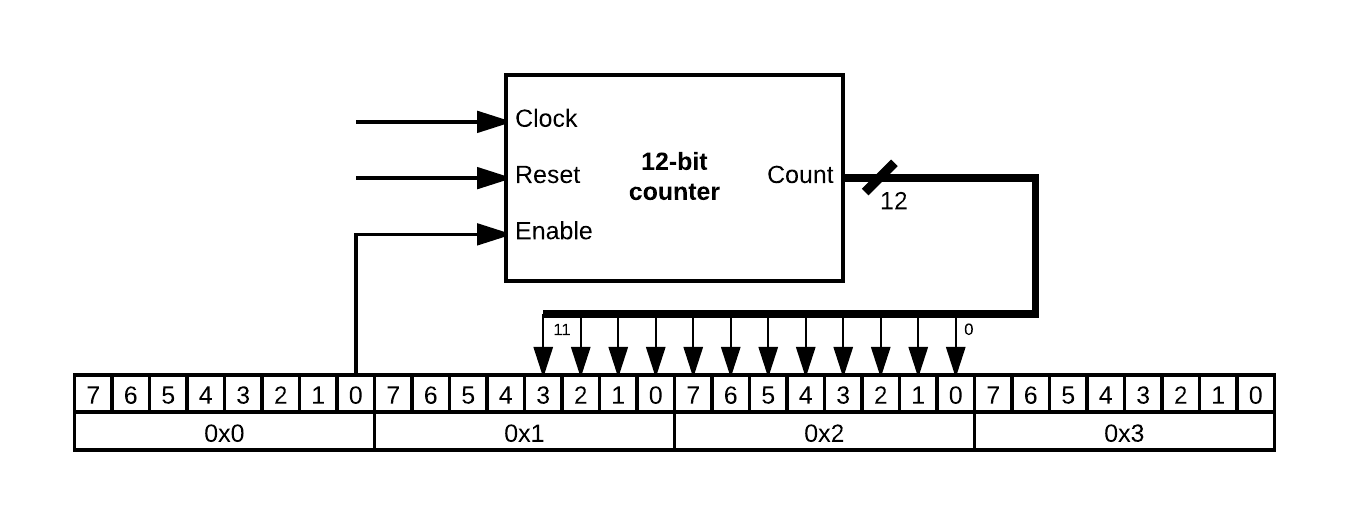
\includegraphics[width=\textwidth]{img/signal-address-projection}
% \end{figure}

% \subsubsection{Output Generation}


\subsubsection{Limitations}
Due to the complexities of the VHDL language, support for a number of language features has been omitted. Although there is no limit on the number of ports, entity port types are limited to be of \texttt{std\_logic} or big-endian \texttt{std\_logic\_vector}, as defined in the \texttt{IEEE.std\_logic\_1164} package. Furthermore, no support for generic parameters has been included in the tool's implementation. Although these limitations may prove to be problematic in production environments, their effects are not considered to be relevant in establishing a proof of concept. These types are among the most commonly used and this limitation can be easily overcome through simple modifications of the top-level VHDL file. Signals between internal instances are not subjected to these limitations.


% \section{Board Package Specification}
% A format for board packages has been developed to facilitate the encapsulation and re-use of FPGA development board-specific logic. This specification is similar to the experiment setup package specification as described in section \ref{section:experiment-setup-package-specification}. The package's unit of containment is also a \texttt{.zip} file archive and has a file structure identical to that displayed in figure \ref{fig:experiment-setup-package-filesystem}. The board package manifest contains package metadata and describes the file contents of the file archive so that the correct files can automatically be selected during the composition process. 

% \begin{lstlisting}[caption={Example board package \texttt{manifest.yaml}}, label={lst:board-package-manifest}]
% type: board-package
% version: 1
% title: Digilent Nexys 4 Board Package
% description: >
%     Board package for Digilent Nexys 4 FPGA Development Board. 
%     PC communication via built-in USB port which emulates a
%     RS232 connection.
% author: Matthijs Bos
% date: (*@ \today @*)
% url: https://github.com/matthijsbos/nexys4boardpackage/
% files: 
%     - ./main.vhd
%     - ./controller.vhd
%     - ./uart.vhd
%     - ./data-link.vhd
% topLevelFile: ./main.vhd
% constraintsFile: ./constraints.
% \end{lstlisting}

% The entity definition for the board package's top-level VHDL file is 

% \begin{lstlisting}[language=vhdl, caption={Top-level VHDL file entity specification.}]
% entity BoardPackage is
%     generic (
%         DATA_WIDTH: integer;
%         ADDRESS_WIDTH: integer);
%     port (
%       clk, reset: in STD_LOGIC;
%       F : out STD_LOGIC);
% end entity BoardPackage;
% \end{lstlisting}


\section{Digilent Nexys 4 Controller}
A controller has been developed for the Digilent Nexys 4 FPGA development board, displayed in figure \ref{fig:nexys4}. The board's primary component is a member of the Xilinx Artix-7 family of FPGAs. An important peripheral component is a controller that allows for the FPGA to be configured over USB, as well as the establishment of a virtual serial point-to-point connection over the same USB connection.

\begin{figure}[h]
\centering
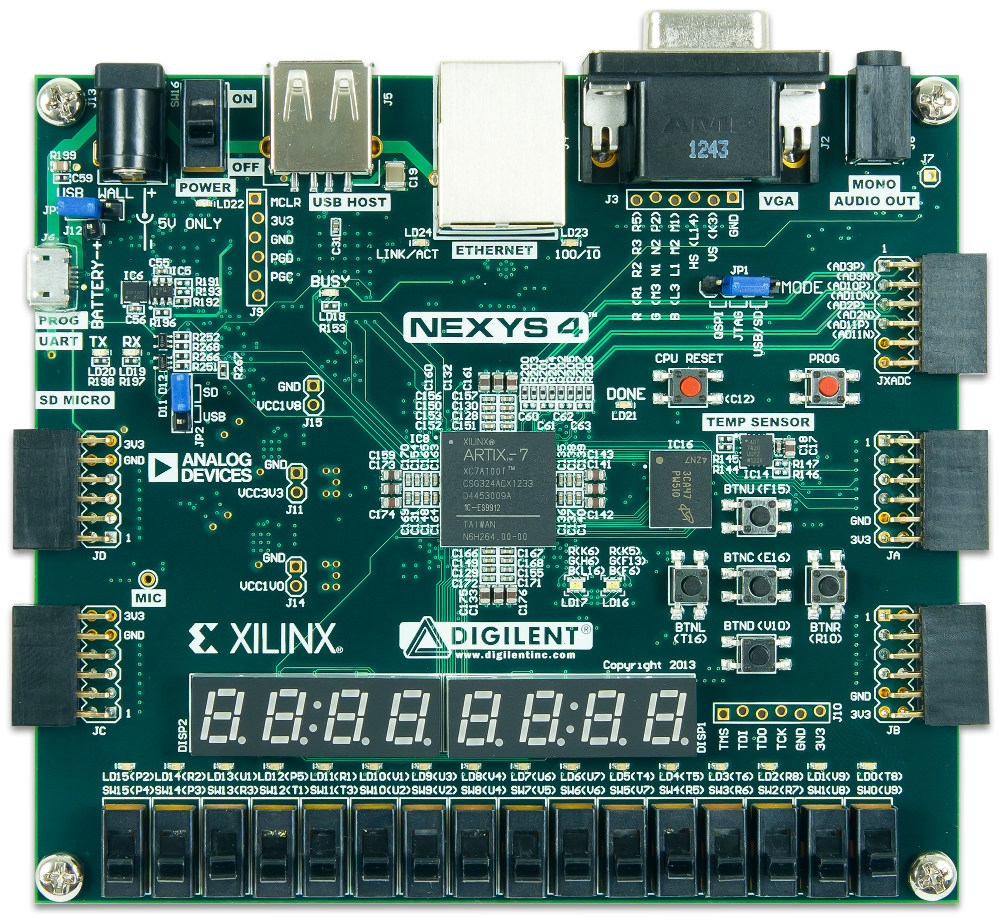
\includegraphics[width=0.5\textwidth]{img/nexys4-small}
\caption{Digilent Nexys 4 Artix-7 FPGA development board}
\label{fig:nexys4}
\end{figure}

% \begin{figure}[h]
% \centering
% 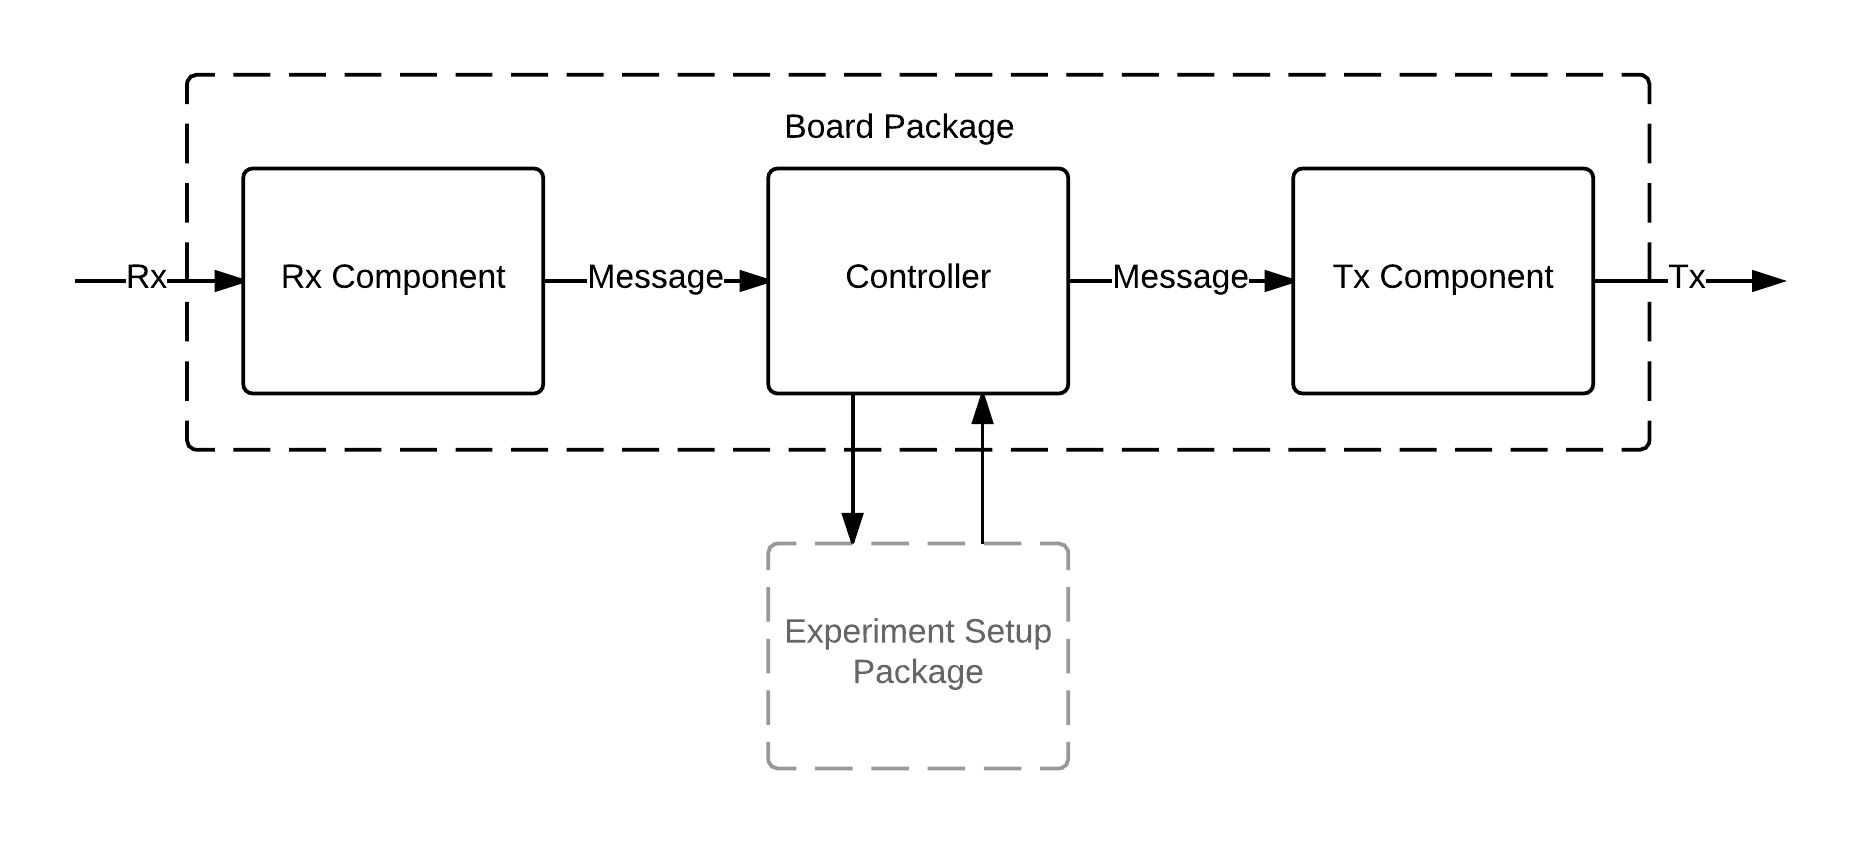
\includegraphics[width=\textwidth]{img/board-package-overview}
% \caption{An overview of the board package logic architecture.}
% \label{fig:board-package-overview}
% \end{figure}


\subsection{Communication Protocol}
\label{section:communication-protocol}
A communication protocol has been designed to facilitate communication between the PC and the Controller embedded in the FPGA. When considering the OSI model as described in \cite[p.28]{tanenbaumcomputer}, the protocol exists in the physical and data link layers. Furthermore, an application layer has been defined. 
% Figure \ref{fig:communication-osi} displays an overview of the protocol stack. 
Since the communication channel is established on a point-to-point basis and does not require any mechanisms for reliable communication, any layers in between have not been considered relevant.

% \begin{figure}[h]
% \centering
% 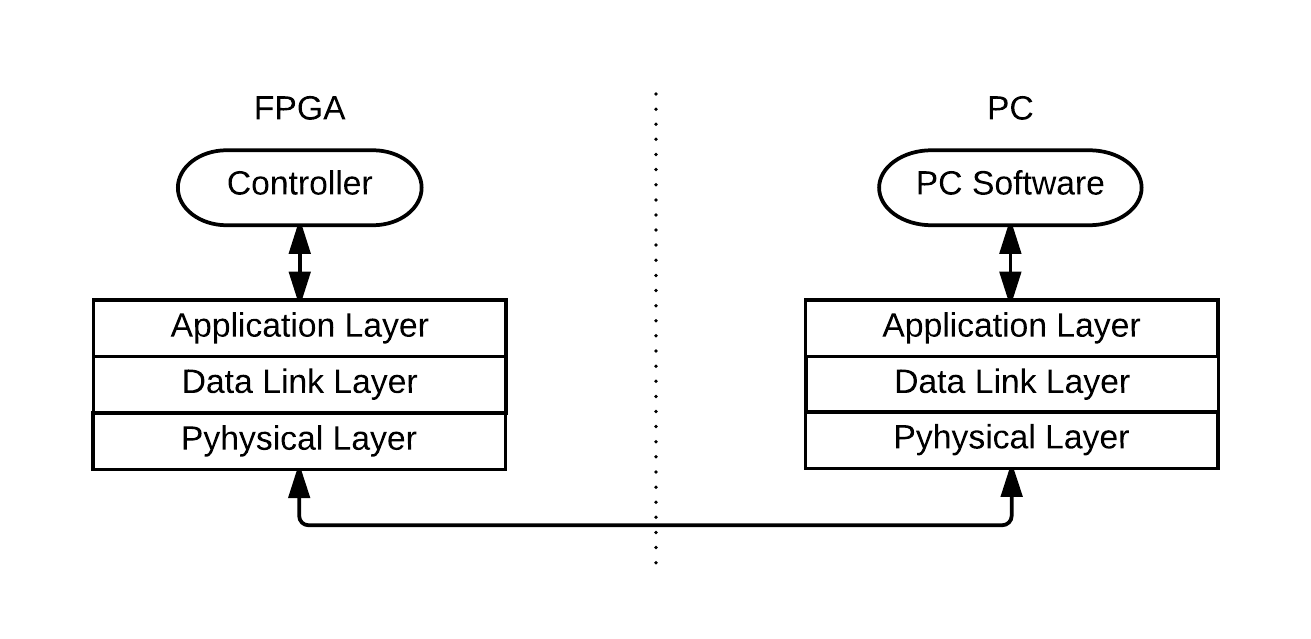
\includegraphics[width=0.6\textwidth]{img/communication-osi}
% \caption{An overview of the communication protocol's layered structure.}
% \label{fig:communication-osi}
% \end{figure}

\subsubsection{Physical Layer}

On the physical layer, the FPGAs peripheral devices facilitate a large part of the communication between the controller and PC. As described in \cite[p.9]{nexys4reference}, the Nexys 4 board features dedicated hardware for communication with the PC through a USB-UART bridge. A Rx and Tx line are available to specific FPGA pins and a virtual "COM" ports is made available on the user's PC. As part of the logic design embedded in the FPGA, another UART\footnote{Universal Asynchronous Receiver/Transmitter} is used in order to receive data from and transmit data to the PC. Although the board features other means of machine-to-machine communication such as Ethernet, the approach involving UARTs was chosen for reasons of simplicity and compatibility.

\subsubsection{Data Link Layer}
UARTs typically handle byte-sized units. In order to support the transmission and reception of larger units of data, a simple data-link layer has been implemented in order to define a data frame. To minimize the complexity of the implementation, the decision was made to provide an unacknowledged and  connectionless service, as described in \cite[p.177]{tanenbaumcomputer}. Although a production-oriented implementation might benefit from more robustness in the data-link layer, features such as frame acknowledgement and error detection have not been considered relevant in establishing a proof of concept. Due to the current implementation's adoption of the layered OSI model however, it should be possible to modify the data link layer to support these features. 

In order to identify individual frames of data, character stuffing \footnote{Also known as byte stuffing.} is used, as described in \cite[p.180]{tanenbaumcomputer}. Specific byte values are assigned to flag a frame's start and end. An escape character is used to prevent frame data to be identified as a control character. As in \cite{Frami37}, character \texttt{0x12} is used as a start flag, \texttt{0x13} as a stop flag and \texttt{0x7D} is used as escape character. Bytes are transmitted in big-endian order. Figure \ref{fig:character-stuffing} displays an example data frame.

\begin{figure}[h]
\centering
\caption{Example data frame for transmission of six bytes: \texttt{0xA1}, \texttt{0xB2}, \texttt{0x12}, \texttt{0xB2}, \texttt{0x7D}, \texttt{0xB2}. The third and fifth byte are preceded by escape character \texttt{0x7D}.}
\label{fig:character-stuffing}
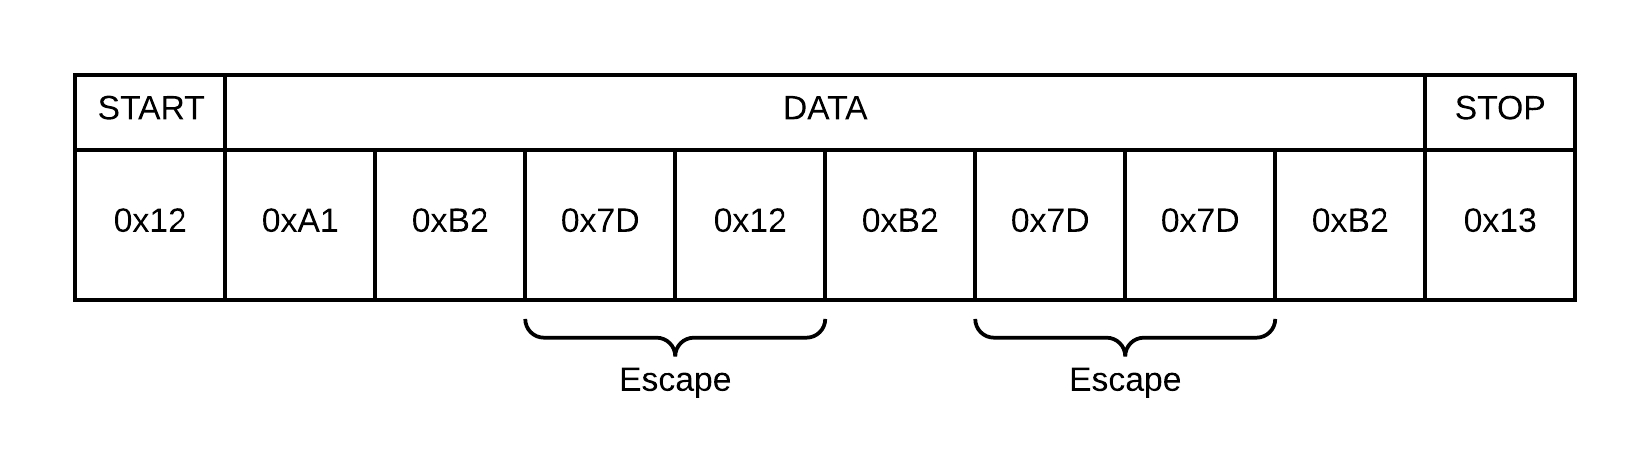
\includegraphics[width=.8\textwidth]{img/character-stuffing}
\end{figure}

\subsubsection{Application Layer}

On the application layer, a message format has been defined, similar to a processor's instruction set as described in \cite{hennessy2013computer}, for example. Messages have a fixed width and conform to be either an address-type or value-type message, as displayed in figure \ref{fig:message-formats}.  Both message types reserve their most significant byte position for the message opcode, a term commonly used in instruction sets to identify an instruction's desired operation. The two message formats suffice in covering the variations that exist in the different message types. Address-type messages are used to interact with the experiment setup's address space, while the value-type message format is used to describe the other operations. Both controller command and response messages use the same formats. 

\begin{figure}[h]
    \centering
    \caption{Message formats for a controller with an address width of 32 and a data width of 8.}
    \label{fig:message-formats}    \begin{subfigure}[t]{\textwidth}
        \centering
        \caption{Address-type message format}
        \label{fig:message-format-address-typed}
        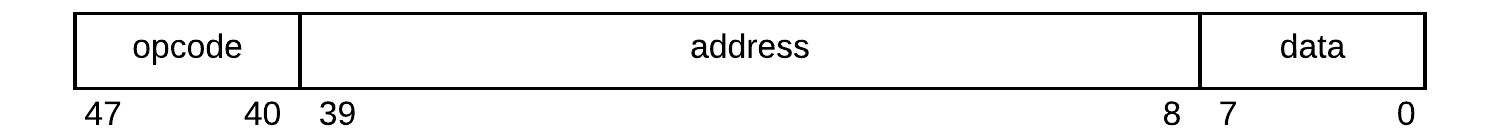
\includegraphics[width=0.75\textwidth]{img/message-format-address-typed}%
    \end{subfigure}
    \begin{subfigure}[t]{\textwidth}
        \centering
        \caption{Value-type message format}
        \label{fig:message-format-value-typed}
        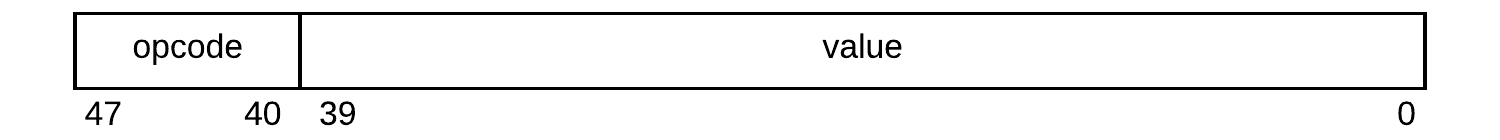
\includegraphics[width=0.75\textwidth]{img/message-format-value-typed}%
    \end{subfigure}

\end{figure}

Tables \ref{tbl:opcodes-cmd} and \ref{tbl:opcodes-res} list the available opcodes for controller commands and responses respectively. The command opcodes have been chosen to reflect the operations that are exposed from the controller to the PC software. As can be observed from these tables, a large number of operations do not require to pass information as arguments. One might argue that a variable-length message format could have been more appropriate. In this implementation however, the decision was made to focus on simplicity and a fixed-length approach was taken to allow for simple message processing logic in the controller.

Some controller responses have a counterpart that is defined to indicate an error in the processing of the requested command. These errors represent the error of being incapable of executing the command due to the mode in which the controller is currently operating. The controller is incapable of executing the \texttt{Step (0x3)} command for example, when operating autonomously as the result of a previous \texttt{Start (0x4)} command. A response message with opcode \texttt{Step error (0x6)} would be returned in that case. 

\setlength{\tabcolsep}{8pt}
\renewcommand{\arraystretch}{1.2}

\begin{table}[h]
    \footnotesize
    \caption{Controller commands}
    \label{tbl:opcodes-cmd}
    \centering
    \begin{tabular}{|l|l|l|l|}
        \hline
        \textbf{Name} & \textbf{Opcode} & \textbf{Type} & \textbf{Arguments}    \\ \hline
        Read          & 0x00            & Address-type  & Address               \\
        Write         & 0x01            & Address-type  & Address, Data         \\
        Reset         & 0x02            & Value-type    & None                  \\
        Step          & 0x03            & Value-type    & None                  \\
        Start         & 0x04            & Value-type    & None                  \\
        Pause         & 0x05            & Value-type    & None                  \\
        Status        & 0x06            & Value-type    & None                  \\ \hline
    \end{tabular}
\end{table}
\begin{table}[h]
    \footnotesize       
    \caption{Controller responses}
    \label{tbl:opcodes-res}
    \centering
    \begin{tabular}{|l|l|l|l|}
        \hline
        \textbf{Name}  & \textbf{Opcode} & \textbf{Type}  & \textbf{Arguments}  \\ \hline
        Read Success   & 0x00            & Address-type   & Address, Data       \\
        Read Error     & 0x01            & Address-type   & Address             \\
        Write Success  & 0x02            & Address-type   & Address, Data       \\
        Write Error    & 0x03            & Address-type   & Address, Data       \\
        Reset Success  & 0x04            & Value-type     & None                \\
        Step Success   & 0x05            & Value-type     & Value               \\
        Step error     & 0x06            & Value-type     & None                \\
        Start Success  & 0x07            & Value-type     & Value               \\
        Start Error    & 0x08            & Value-type     & None                \\
        Pause Success  & 0x09            & Value-type     & Value               \\
        Pause Error    & 0x0A            & Value-type     & None                \\
        Status Success & 0x0B            & Value-type     & Value               \\ \hline
    \end{tabular}
\end{table}

% \subsubsection{Message Format Parametrization}

% An experiment setup's address and data buses have a variable width and the controller must thus match these specifications. While one experiment setup might require address and data buses of 2 and 1 bits wide respectively, another might require an address bus and data bus of 32 bits wide. Not only must the controller support scaling in order to support these changes, its message formats must be parametrized as well. As a consequence, message formats might vary for different compositions of board and experiment setup packages. 
% % Since the widths of these buses are known at compile-time, the parametrization 

% In order to support this dynamic behaviour, the boundaries between different sections of the message must be determined based on the width definitions for the address and data buses of the experiment setup package. The equations displayed in figure \ref{fig:message-parametrization-equations} define how other message format parameters are expressed in terms of the widths of these buses. Every section is defined to span at least one byte. As a result, the minimum message width is defined to be three bytes wide. This decision was made to allow for simplified debugging and processing on the PC, since a byte corresponds to a PC's unit of memory and sections can thus be easily separated. Furthermore, it guarantees the \texttt{Value} section of value-types messages to have a width of at least 16 bits, large enough for reasonably sized integer representations. If the section is wider than the corresponding signal due to rounding, the unused bits are located on the MSB end of the section and are set to be zero. All arguments represent unsigned integers and are thus unaffected when interpreted as bytes. 


% \begin{figure}[h]
%     \caption{Equations for message format parametrization in terms of $address\ width$ and $data\ width$. Every message section is defined to span at least one byte.}
%     \label{fig:message-parametrization-equations}
%     \centering
%     \begin{empheq}[box=\fbox]{align*}
%     % \begin{align*}
%         \# command\ opcodes     &= 7 \\
%         \# response\ opcodes    &= 12 \\
%         \# opcode\ bytes        &= \bigg \lceil \frac{max(\#command\ opcodes, \#response\ opcodes)}{256} \bigg \rceil = 1\\
%         \# address\ bytes       &= \bigg \lceil \frac{address\ width}{8} \bigg \rceil \\
%         \# data\ bytes          &= \bigg \lceil \frac{data\ width}{8} \bigg \rceil \\
%         \# message\ bytes       &= \# opcode\ bytes + \# address\ bytes + \# message\ bytes \\
%         \# value\ bytes         &= \# address\ bytes + \# data\ bytes \\
%         value\ width            &= 8 \cdot \# value\ bytes
%     % \end{align*}
%     \end{empheq}
% \end{figure}

\subsection{Logic Architecture}
A controller for the Digilent Nexys 4 FPGA development board has been implemented. Figure \ref{fig:board-package-architecture} displays an overview of the controller's logic architecture. The architecture features the logic for experiment setup control as well as logic that implements a communication protocol described in section \ref{section:communication-protocol}. The controller source code is made available through a git repository \footnote{\url{https://github.com/matthijsbos/fpgaedu-nexys4-python}}. The logic architecture has not been directly implemented using VHDL, but was modeled in Python code through the MyHDL\footnote{\url{http://www.myhdl.org/}} library. The choice for MyHDL was made to allow for increased agility during development and its capabilities for fast and efficient unit testing of components. The library allows for automatic conversion of Python sources to VHDL, so it only serves as an intermediary representation during development.

\begin{figure}[h]
\centering
\caption{An overview of the Nexys 4 board package logic architecture, largely following the conventions for representation as defined in \cite[Ch.4]{hennessy2013computer}. The experiment setup component's address and data buses are defined to have widths of 32 and 8 bits respectively.}
\label{fig:board-package-architecture}
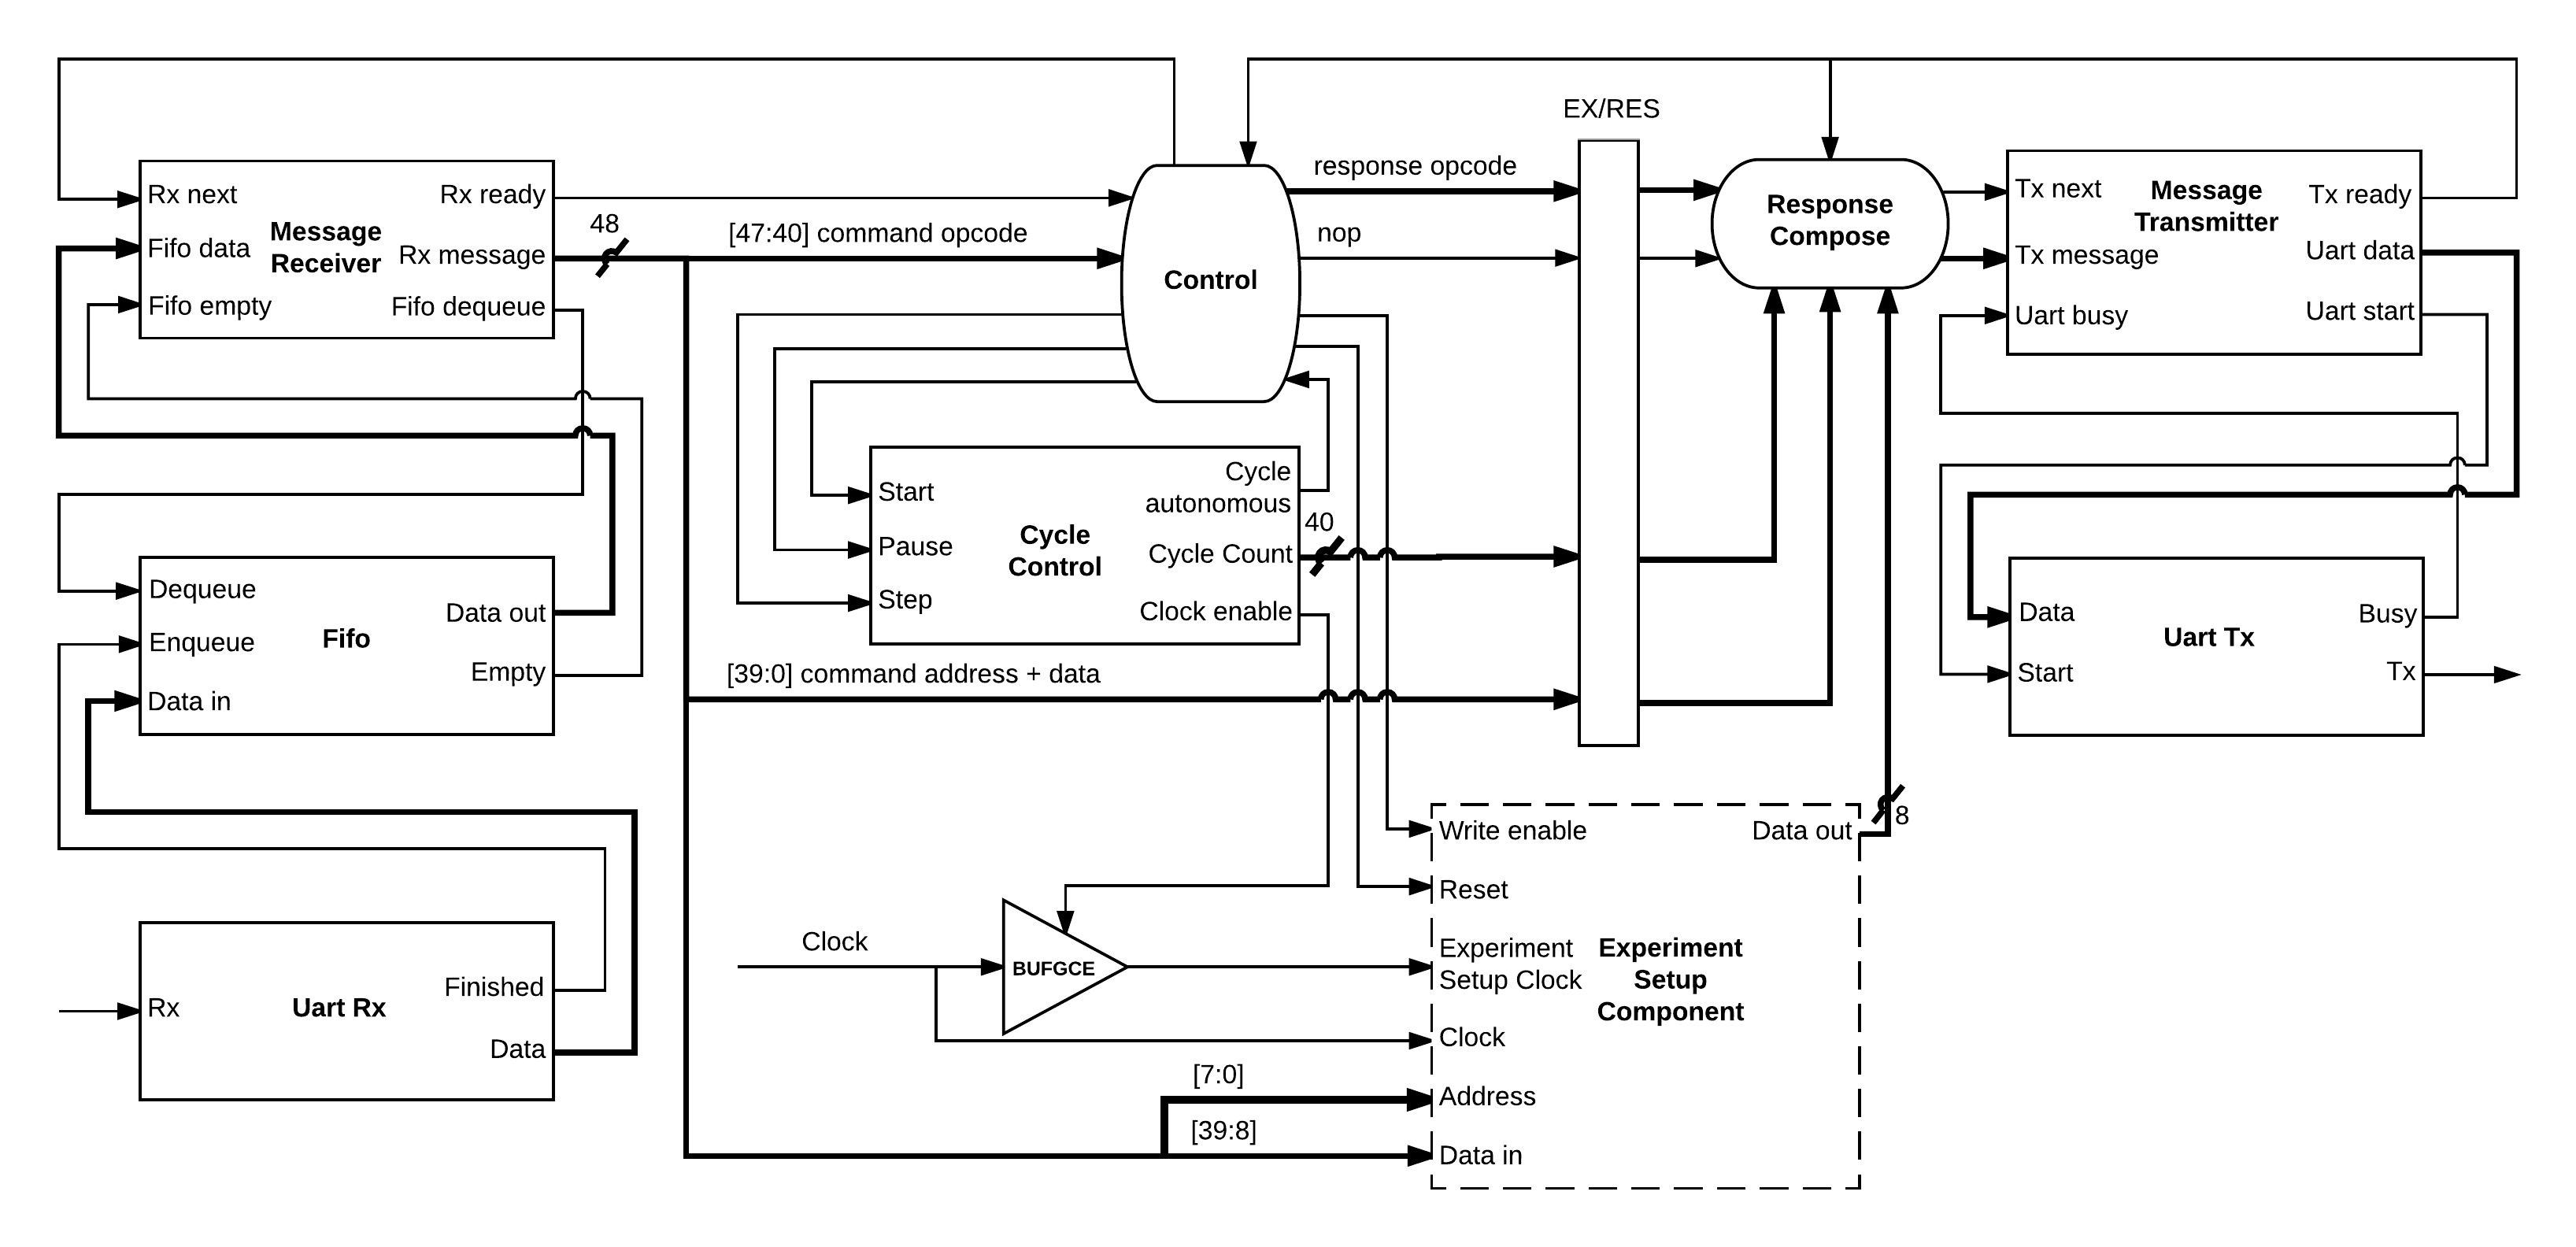
\includegraphics[width=\textwidth]{img/controller-architecture}
\end{figure}

\subsubsection{PC Communication}

On the physical layer, a standard UART has been implemented for both reception and transmission of bytes. The receiving UART writes to a buffer, since command messages have a length of multiple bytes. No error detection operations are performed, since it has not been considered relevant in establising a proof of concept. The data link layer has been implemented in the message receiver and message transmitter components. The message receiver component reads from the buffer until a valid data frame is identified through its flags. Once a complete frame has been received, the component notifies the controller of the reception of a new command message. The message is held in an internal register until the controller has signaled the receiver component to start receiving a new data frame, and thus serves as an additional buffer. 

Once the controller is ready to transmit a response message to the PC, the message's contents are written to the message transmitter's internal register and the transmitter is signalled to start transmission. During transmission, the message transmitter serves as a buffer for outgoing messages. The transmitter component then sequentially instructs the transmitting UART to transmit the response message's contents, automatically inserting control flags and escaping reserved characters. 

\subsubsection{Controller}
The logic for controlling the experiment setup as displayed in figure \ref{fig:board-package-architecture} is collectively referred to as the controller. More specifically, it concerns the blocks of combinational logic labeled \texttt{Control} and \texttt{Response Compose}, as well as the block of sequential logic labeled \texttt{Cycle Control} working in conjunction with a \texttt{BUFGCE} clock buffer. THe \texttt{BUFGCE} clocking resource is described in \cite[p.40]{ug472}. The components are divided over the two stages execute (\texttt{EX}) and response (\texttt{RES}), which are connected through a pipeline register \texttt{EX/RES}.

The \texttt{Control} block is responsible for setting control signals based on incoming commands, as well as receiver and transmitter status signals. Furthermore, the block is responsible for determining the opcode for the response message based on the incoming command as well as the current mode of operation (manual or autonomous). This approach to defining control signals is similar to that taken in \cite[Ch.4]{hennessy2013computer}. As the name suggests, the \texttt{Response Compose} block is responsible for composing a response message from different sources based on the response opcode, as well as signalling the message transmitter to initiate transmission of a new message.

As can be observed from figure \ref{fig:board-package-architecture}, the experiment setup's input signals have different origins. Most input signals are derived from the incoming command message, but the clock signal is driven by a \texttt{BUFGCE} clock gating buffer. This type of component is specific to Xilinx FPGAs. In its turn, the clock buffer's \texttt{Clock enable} signal is controlled by the \texttt{Setup Cycle Control} component. All sequential logic in the architecture is positive-edge-triggered, except for the logic driving the \texttt{Clock enable} signal. This approach of negative-edge-triggered logic was taken to ensure predictable timing for the clock edges of the gated clock signal. Figure \ref{fig:timing-cycle-control} displays a timing diagram for the \texttt{Cycle Control} component working in combination with the \texttt{BUFGCE} clock buffer. By enabling the \texttt{Clock enable} signal while the clock signal is low, no unexpected edges will occur. The same applies to the disabling of the \texttt{Clock enable} signal. 

\begin{figure}[h]
\centering
\caption{Timing diagram for the \texttt{Cycle Control} logic block in combination with the \texttt{BUFGCE} clock buffer.}
\label{fig:timing-cycle-control}
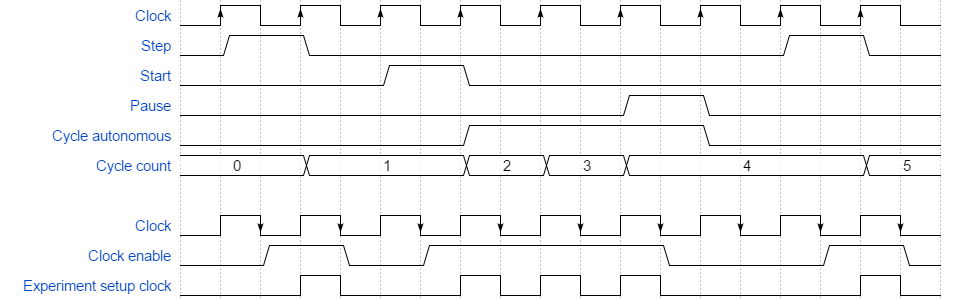
\includegraphics[width=\textwidth]{img/cycle-control}
\end{figure}

As described in section \ref{sectioncontrollerabstraction}, the experiment setup is defined to take one clock cycle to perform read and write operations. In order to allow for this delay, a pipeline register was introduced to temporarily store the values passed from the \texttt{execute} stage to the \texttt{response} stage, as well as to handle the single cycle delay introduced by the negative-edge-triggered approach to gating the \texttt{experiment setup clock} signal.

\section{Experimentation Package Specification}
A format for the model's experimentation packages has been defined. This specification is similar to the experiment setup package specification as described in section \ref{section:experiment-setup-package-specification}. The package's unit of containment is also a \texttt{.zip} file archive and has a file structure identical to that displayed in figure \ref{fig:experiment-setup-package-filesystem}. The experimentation package's manifest contents are mostly similar to that of the experiment setup pacakge's. It contains experiment setup metadata, as well as a description of the experiment setup's address space. Since the experimentation package is targeted at a specific FPGA development board, its manifest contains a description of this development board as well. In stead of referring to the source vhdl files, the manifest contains a file pointer to the bitstream file contained within the package. 

\section{Digilent Nexys 4 Composer}
In order to facilitate the model's component composition process as described in section \ref{sectioncomponentcomposition}, a tool has been developed that automates this task. Similar to the experiment setup wrapper as described in section \ref{section:experiment_setup_wrapper}, this tool is implemented using the Java 8 programming language and its source code is made available through a git repository\footnote{\url{https://github.com/matthijsbos/fpgaedu-java}}. The tool is activated through the command line by the command \texttt{fpgaedu compose}.

The tool takes an experiment setup package as an input and extracts the experiment setup package's source files. The package's top-level file is parsed to extract its entity and architecture identifiers. This information is then used in the generation of a new top-level vhdl file that composes the experiment setup's sources and the controller sources to form a complete set of board-specific sources. A contraints file is then generated to match FPGA pins to the new top-level file's input and output signals.

In order to activate the FGPA's toolchain, a new script is then generated for the Xilinx Vivado SDK. This script instructs Vivado which files to include in the set of sources, as well as wihch specific FPGA model is to be targeted. Once generated, the script is executed in the background and a new bitstream is generated by Vivado. On successful execution, the bitstream is then packaged into an experiment setup package, together with a definition of the experiment setup's address space.

% \section{Experimenter Shell}
% A simple shell has been developed such that the controller may be operated. 


\end{document}